% !TEX TS-program = pdflatex
% !TEX encoding = UTF-8 Unicode

% TeX-M (r1.1)
% For my math classes at UT Austin
% Notes template created by Abdon Morales for the College of Natural Science
% and for the Department of Mathematics and Computer Science
% (c) 2019 - 2024 Abdon Morales and the University of Texas at Austin
% This is a notes template for a LaTeX document using the "article" class for Mathematics (Calculus)
% at the University of Texas at Austin.

% Last change made: Jan 27, 2024 1:40 AM CST

% See "book", "report", "letter" for other types of document.

\documentclass[11pt]{article} % use larger type; default would be 10pt

% Start of Article customization options and addons (for more help and information reference to Overleaf's guides and docs on Latex.
\usepackage[utf8]{inputenc} % set input encoding (not needed with XeLaTeX)

%%% Examples of Article customizations
% These packages are optional, depending whether you want the features they provide.
% See the LaTeX Companion or other references for full information.

%%% PAGE DIMENSIONS
\usepackage{geometry} % to change the page dimensions
\geometry{letterpaper} % or letterpaper (US) or a5paper or....
% \geometry{margin=2in} % for example, change the margins to 2 inches all round
% \geometry{landscape} % set up the page for landscape
%   read geometry.pdf for detailed page layout information

\usepackage{graphicx} % support the \includegraphics command and options
\usepackage{xcolor}

% \usepackage[parfill]{parskip} % Activate to begin paragraphs with an empty line rather than an indent

%%% PACKAGES
\usepackage{booktabs} % for much better looking tables
\usepackage{array} % for better arrays (eg matrices) in maths
\usepackage{paralist} % very flexible & customisable lists (eg. enumerate/itemize, etc.)
\usepackage{verbatim} % adds environment for commenting out blocks of text & for better verbatim
\usepackage{subfig} % make it possible to include more than one captioned figure/table in a single float
\usepackage{exercise}
% Math tools
\usepackage{mathtools}
\usepackage{amsmath}
\usepackage{tikz} % For charts, mathematical graphs, and etc
%% Equal symbol for L'Hospital Rule
\usepackage{tcolorbox}
\newcommand\LR{\stackrel{\mathclap{\normalfont\mbox{L.R}}}{=}}
% These packages are all incorporated in the memoir class to one degree or another...

%%% HEADERS & FOOTERS
\usepackage{fancyhdr} % This should be set AFTER setting up the page geometry
\pagestyle{fancy} % options: empty , plain , fancy
\renewcommand{\headrulewidth}{0pt} % customise the layout...
\lhead{}\chead{}\rhead{}
\lfoot{}\cfoot{\thepage}\rfoot{}

%%% SECTION TITLE APPEARANCE
\usepackage{sectsty}
\allsectionsfont{\sffamily\mdseries\upshape} % (See the fntguide.pdf for font help)
% (This matches ConTeXt defaults)

%%% ToC (table of contents) APPEARANCE
\usepackage[nottoc,notlof,notlot]{tocbibind} % Put the bibliography in the ToC
\usepackage[titles,subfigure]{tocloft} % Alter the style of the Table of Contents
\renewcommand{\cftsecfont}{\rmfamily\mdseries\upshape}
\renewcommand{\cftsecpagefont}{\rmfamily\mdseries\upshape} % No bold!
%%% Question creation
\renewcommand\ExerciseName{Question~}
\renewcommand\AnswerName{Answer to question}
\renewcommand\ExerciseHeader{%
  \noindent\parbox[t]{.18\textwidth}{%
    \bfseries\large\ExerciseName\ExerciseHeaderNB\hfill}%
  \parbox[t]{.72\textwidth}{%
    \centering\bfseries\large%
    \ExerciseHeaderTitle\ExerciseHeaderOrigin}%
  \par\medskip
}
%%% END Article customizations

%%% The "real" document content comes below...

\title{The Aggregate Demand-Aggregate Supply Model}
\author{Abdon Morales \\ The University of Texas at Austin \\ ECO 304L: Introduction to Macroeconomics \\ Wayne Geerling}
\date{\today \\ Chapter 13 : Week 7}
%\date{} % Activate to display a given date or no date (if empty),
         % otherwise the current date is printed 

\begin{document}
\maketitle
\subsection*{The economy does not follow a predictable cycle of expansion and contraction.}
In March 2020, the global economy fell off a cliff, plunged into turmoil by the coronavirus pandemic. Prior to the outbreak, the American economy had been in its longest expansion on record, with the unemployment rate below 4\%. Then output plummeted, and the unemployment rate rose to almost 15\% by April. Oddly, some analysts had been warning in the months prior of an impending recession; while they didn't foresee a pandemic, they predicted a downturn simply because it had been so long since the last recession.

Many consider the pattern of economic ups and downs to be inevitable; the term "business cycle" is a popular way to describe the recession-expansion phenomenon, because so many people are convinced that the recession recession-expansion pattern occurs in a regular cycle. Yet, despite recent turmoil, recessions are relatively rare; while there have been 23 U.S recessions since 1900 and only four since 1982. Complicating matters, no two recessions are exactly alike in cause or effect.

If your interest in macroeconomics stems from a desire to learn more about recessions and their causes, this is the chapter for you. In this chapter we focus on short-run fluctuations in the macroeconomy and build a model that helps us understand why they happen. This model will also help us see how the three big macroeconomic variables discussed in earlier chapters, namely GDP, unemployment, and inflation, fit together.

\begin{tcolorbox}[width=\textwidth,colback={white},title={Big Questions},colbacktitle=yellow,coltitle=blue]
\begin{itemize}
\item What is the aggregate demand-aggregate supply model?
	\subitem \textbf{-} The aggregate demand-aggregate supply model is a model that economists use to study business cycles (short-run fluctuations in the economy).
\item What is aggregate demand?
	\subitem \textbf{-} Aggregate demand represents the spending side of the economy. It is the total demand for final goods and services in an economy; it also includes consumption, investment, government spending, and net exports.
	\subitem \textbf{-} The slope of the aggregate demand curve is negative due to the wealth effect, the interest rate effect, and the international trade effect.
	\subitem \textbf{-} The aggregate demand curve shifts when there are changes in consumption factors (real wealth, expected future income, taxes), investment factors (firm confidence, interest rates, the quantity of money), government spending (at federal, state, and local levels), or net export factors (foreign income and the value of the U.S dollar).
\item What is aggregate supply?
	\subitem \textbf{-} Aggregate supply represents the producing side of the economy. It is the total supply of final goods and services in an economy.
	\subitem \textbf{-} The long-run aggregate supply curve is relevant when all prices are flexible; this curve is vertical at full-employment output and is not influenced by the price level.
	\subitem \textbf{-} In the short run, when some prices are sticky, the short-run aggregate supply curve is relevant. This curve indicates a positive relationship between price level and real output supplied.
	\subitem \textbf{-} How does the aggregated demand-aggregated supply model help us understand the economy?
	\subitem \textbf{-} We can use the aggregate demand-aggregate supply model to see how changes in either aggregated demand or aggregate supply (or both) affect real GDP, unemployment, and the price level.
\item How does the aggregate demand-aggregate supply model help us understand the economy?
\end{itemize}
\end{tcolorbox}

\section*{\textbf{What is the aggregate demand-aggregate supply model?}}
In macroeconomics, there are two major paths of study; one direction explores long-run growth and development. The second direction examines short-run fluctuations, or business cycles. The two paths are complementary: both study GDP growth, employment, and the people, firms, and governments that impact the economy; but they are certainly distinct: growth economics focuses on theories and policies that affect economic progress over several decades, whereas business cycle theory typically focuses on times horizons of five years or less.

In Chapter 6, we presented the idea of a basic business cycle, in which real GDP increases for a while during the expansionary phase and then decreases during the contractionary, or recessionary, phase. The business cycle is most evident in real GDP growth and unemployment rates. During recessions, real GDP growth slows and the unemployment rate rises; during expansions, real GDP growth expands and the unemployment rate falls.

Panel (a) of Figure 13.1 shows real GDP growth rates by quarter for the United States from 1990 to 2021. The blue vertical bars indicate four recessions during this period. Panel (b) plots the unemployment rate over the same period; the unemployment rate rose sharply during each of the recessions and then fell afterward. The highest unemployment rate during this period was 14.7\% in April 2020.

\begin{center}
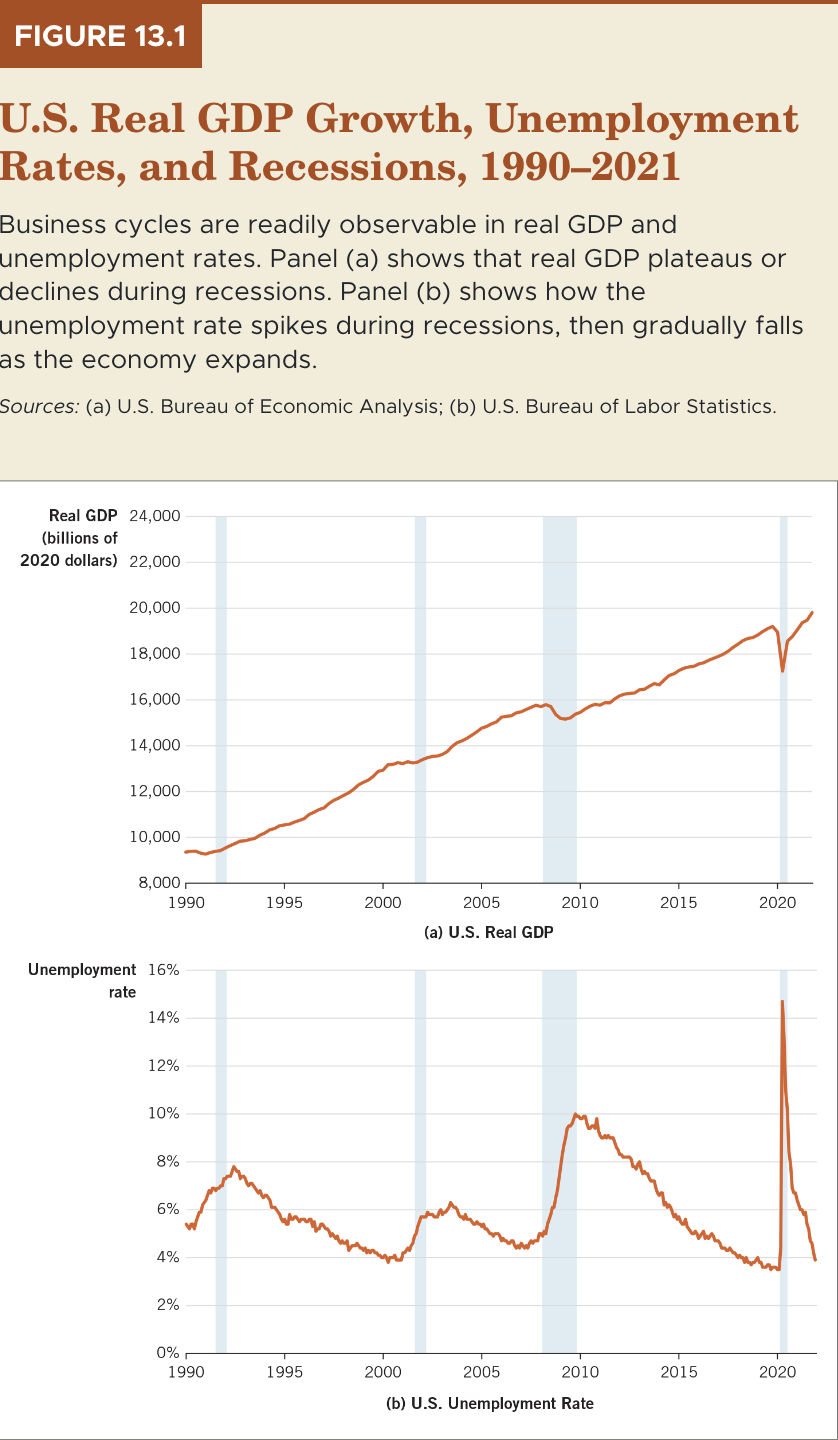
\includegraphics[scale=0.4]{images/Figure 13.1.png}
\end{center} 

The model we use to study business cycles is the aggregate demand-aggregate (AD-AS) supply model. At the core of the model are the familiar concepts of demand and supply; in earlier chapters, we looked at the demand and supply of a single good, like pizza or gasoline. Now we consider demand and supply of all final goods and services in an economy - the demand for and supply of GDP. \textbf{Aggregate demand} is the total demand for final goods and services in an economy. \textbf{Aggregate supply} is the total supply of final goods and services in an economy; the word "aggregate" means total.

We consider each side of the economy separately before bringing them together. The next section explains aggregate demand, and then we turn to aggregate supply.

\section*{\textbf{What is aggregate demand?}}
Here is something you might ask a few people: \textit{How can you personally help our economy?} We predict that most responses will focus on buying something or spending money somewhere. In our model of the economy, this is demand; aggregate demand is the spending side of the economy. When people spend more on goods and services, aggregate demand increases, and most people believe that this spending is what drives the economy. As we'll see, this is only partly true.

To determine aggregate demand, we sum up spending from different sources in the economy. These sources include private domestic consumers who buy cars, food, clothing, education, and other goods and services. Business firms are another major group; they buy resources needed to produce output. The government is a third large purchaser of labor and other resources used to produce government services. Finally, foreign consumers buy many goods and services produced in the United States. These four major groups constitute the four pieces of aggregate demand: consumption (C), investment (I), government spending (G), and net exports (NX). The total of these four yields aggregate demand (AD) in a given period:
\begin{equation}
\text{AD} = C + I + G + \text{NX}
\end{equation}
As we study aggregate demand, we consider factors that affect each of these sources. (For a review of C, I, G, and NX, see Chapter 6).

Figure 13.2 shows a graph of the aggregate demand curve; on the horizontal axis, we plot quantities of all final goods and services, which constitute real GDP. On the vertical axis, we measure the overall price level (P) in the economy; this is not the price of any particular good or service, but rather a general level of prices for the whole economy. Because we are looking at all final goods and services, the correct price index to use is the GDP deflator is at 100 (1982-83) in a particular period of time and the fluctuates from that level. A rise in P indicates inflation in the economy.

\begin{center}
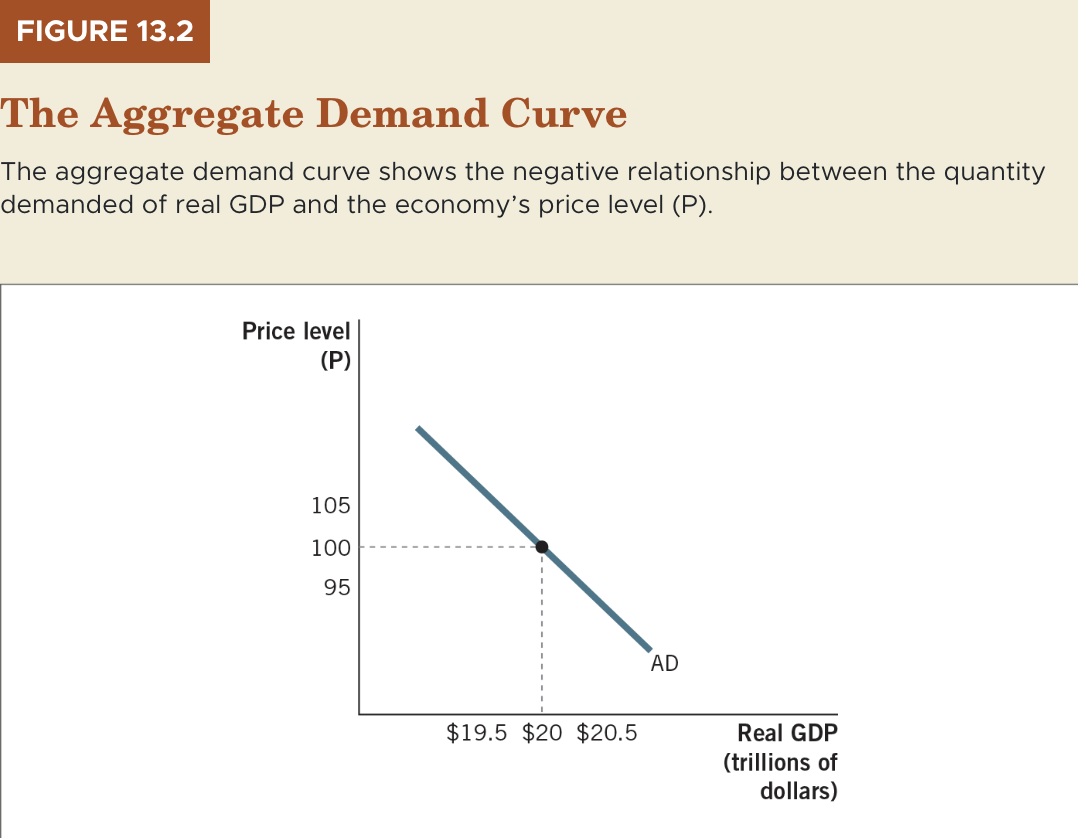
\includegraphics[scale=0.5]{images/Figure 13.2.png} 
\end{center}

On the graph in Figure 13.2, we have labeled a particular point where the price level is 100 and the quantity of aggregate demand is \$20 trillion. The negative slope of the aggregate demand curve means that increases in the price level lead to decreases in the quantity of aggregate demand; when the price level falls, the quantity of aggregate demand rises, but be careful here: aggregate demand does not slope downward for the same reason that individual demand curves slope downward. In this next section, we explain the reasons for the negative slope of the aggregate demand.

\subsubsection*{The Slope of the Aggregate Demand Curve}
All else equal, increases in the price level lead to decreases in the quantity of aggregate demand. You might agree with this statement without closely evaluating it, because it sounds like the relationship between quantity and demanded of a single good and its price; but now we are evaluating the whole economy. Remember that the price level is the general price level of all final goods and services. Aggregate demand and aggregate supply don't just measure the quantity of pizzas demanded and supplied; they measure the production of all firms in all the markets that constitute the economy. Therefore, substitutions from one market to another have no effect on the total amount of output, or real GDP. Substituting out of pizza and into chicken nuggets doesn't change the GDP

There are there reasons for this negative relationship between quantity of aggregate demand and the price level: the wealth effect, the interest rate effect, and the international trade effect.

\subsubsection*{The Wealth Effect}
\textbf{Wealth} is the net value of one's accumulated assets; your wealth is the total net value of everything you own, including the money in your wallet and in your bank accounts. The \textbf{wealth effect} is the change in the quantity of aggregate demand from wealth changes due to price-level changes.

\subsubsection*{The Interest Rate effect}
If the price level rises and real wealth falls, people also save less. Therefore, in addition to the wealth effect, an increase in the price level affects people's savings. When you cut back on savings, your action leads to the interest rate effect; the \textbf{interest rate effect} occurs when a change in the price level leads to a change in interest rates and therefore in every quantity of aggregate demand. Remember that every dollar borrowed requires a dollar saved; therefore, when savings decline, the quantity of investment declines, and this is part of aggregate demand.

Figure 13.3 shows the loanable funds market before and after a decrease in savings. Initially, the demand and supply of loanable funds are indicated by curves \(D\) and \(S_1\), and the equilibrium interest rate is 3\%. If the economy's price level rises, people save less, which shifts supply to \(S_2\); the reduction in supply leads to a higher interest rate of 4\% at which point the quantity of investment falls from \(I_1\) to \(I_2\). Because investment is one piece of aggregate demand, a decrease in investment decreases overall aggregate demand; thus, a change in the price level initiates a cascade of events with the result that firms invest less at higher interest rates because individuals are saving less.

\subsubsection*{The International Trade Effect}
When we draw our aggregate demand curve, the price level and real GDP represent those from the domestic market - in this case the United States. In the context of the world economy, we must also consider U.S prices \textit{relative to} the prices from other countries, and the quantity demanded of U.S goods falls. The \textbf{international trade effect} occurs when a change in the price level leads to a change in the quantity of net exports demanded.

\begin{center}
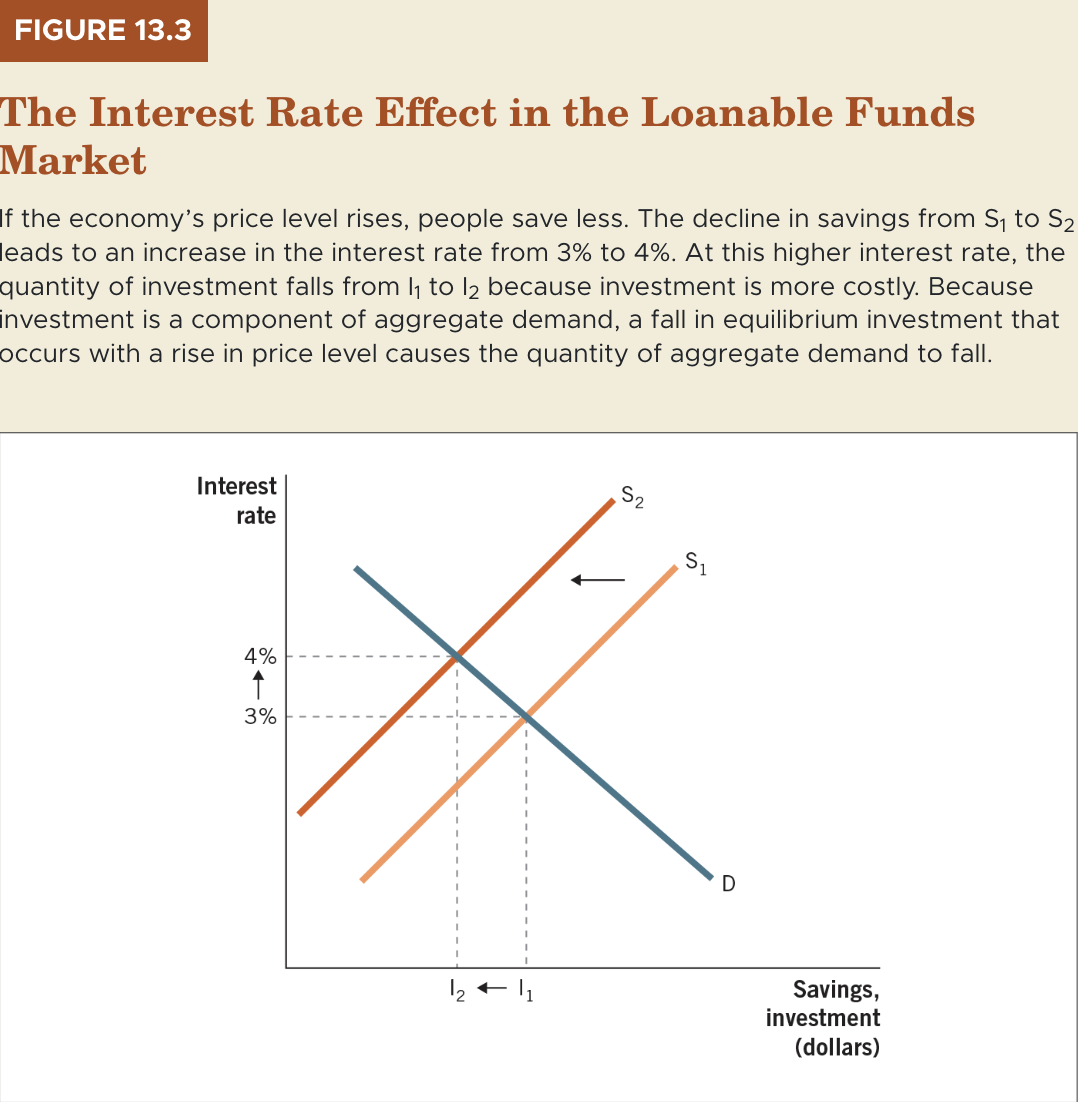
\includegraphics[scale=0.5]{images/Figure 13.3.png} 
\end{center}

Figure 13.4 shows all three effects working together to affect the quantity of aggregate demand; each begins with a change in the economy's price level. When the price level rises from 100 to 110, consumption (C) declines from the wealth effect, investment (I) declines via the interest rate effect, and net exports (NX) fall due to the international trade effect. In reality, the three effects do not influence aggregate demand equally; the international trade effect is relatively small because exports are a relatively small part of the GDP. Because consumption is by far the largest component of GDP, the wealth effect is the most significant.

It is important to distinguish between \textit{shifts in} the aggregate demand curve versus \textit{movements along} the aggregate demand curve. In this section, we have identified three effects related to movements along the aggregate demand curve. These all originate with a change in the economy's price level; in contrast, shifts in the demand curve occur when people demand more, or fewer, goods and services at any given price level. These shifts can come from any of the components of aggregate demand: consumption, investment, government spending, or net exports. In the next section, we consider the factors that shift the aggregate demand curve.

\begin{center}
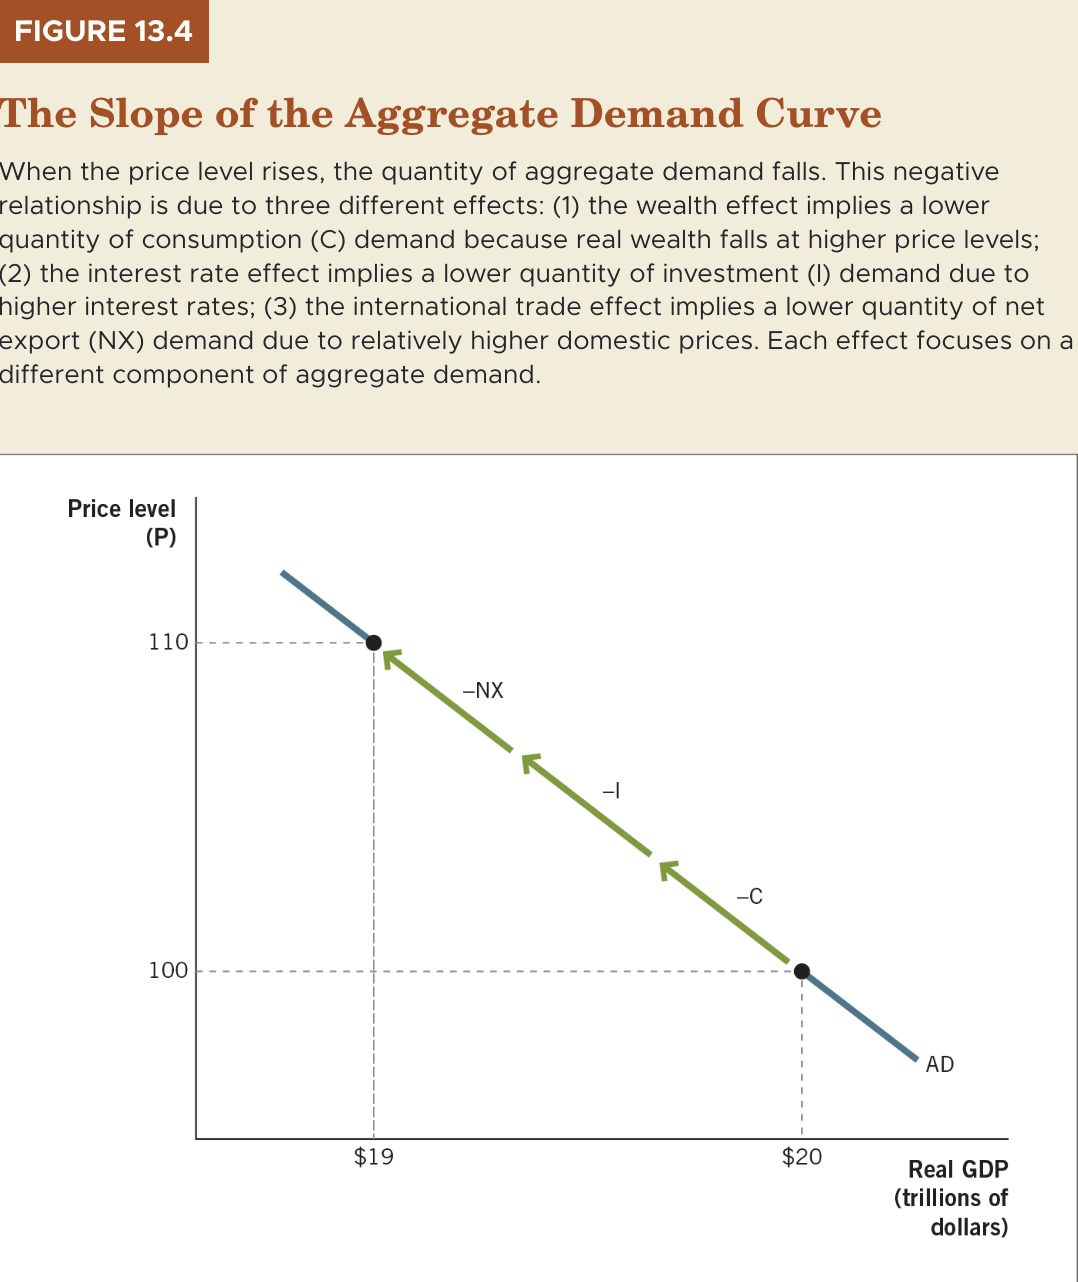
\includegraphics[scale=0.5]{images/Figure 13.4.png} 
\end{center}

\subsection*{Shifts in aggregate demand}
When people demand more goods and services at all price levels, aggregate demand increases and the AD curve shifts to the right. When people demand fewer goods and services at all price levels, aggregate demand decreases and the AD curve shifts to the left.

In thinking about the many factors that shifts aggregate demand, it is helpful to categorize them into the different types of aggregate demand spending: consumption (C), investment (I), government spending (G), and net exports (NX). We begin with factors that cause changes in consumption spending.

\subsubsection*{Shifts in consumption}
Consumption spending accounts for about 70\% of all spending in GDP. In this section, we cover three factors that shift consumption spending; the first is people's current wealth. When national wealth increases, the consumption component of aggregate demand increases; when wealth falls, consumption declines.

Before moving on, we should clarify that here we are talking about changes in individuals' wealth \textit{not} caused by changes in the price level. When we discussed the slope of the aggregate demand curve, we talked about the wealth effect, which is caused by changes in the economy's price level (P). The wealth effect causes a \textit{movement along} the AD curve, not a shift of the AD curve.

Expected future income is a second factor that shifts consumption spending; when people expect higher income in the future, they spend more today.

Pehaps you've heard of the consumer confidence (or consumer sentiment) index; this index, which uses survey data to estimate how consumers feel about the future direction of the economy, is essentially a measure of expected future income. Confidence, or lack of confidence, in the economy's future changes consumer spending today; consumer confidence can swing up or down with unpredictable events such as national elections or international turmoil. When these sentiments change, they change consumption spending and shift the aggregate demand curve.

Finally, taxes also affect consumption spending; when consumers pay lower taxes, they can afford to spend more. When taxes rise, consumers have less to spend; in Chapter 16, we cover the effect of taxes on consumption in greater detail. For now, we note that higher taxes lead to lower consumption and lower aggregate demand.

\subsubsection*{Shifts in investment}
In this section, we consider four factors that shift investment demand. Investment shifts when decision-makers at firms decide to increase or decrease spending on capital goods. One possibility is that business firm confidence changes; keep in mind that in macroeconomics, business firms are the investors, when they spend on plant and equipment used in future production. When firms decide that the future of their industry or the overall economy is positive, they might decide to purchase tools to increase production and future profits. On the other hand, decreases in the business firm confidence lead to decreases in investment and decreases in aggregate demand.

Interest rates also shifts investment demand; an increase in interest rates makes investment more expensive for firms, decreasing aggregate demand. In contrast, lower interest rates decrease the cost of borrowing for firms and increase the investment component of aggregate demand. While we typically focus on investment effects from interest rate changes, consumption is also affected by changes in interest rates. At lower interest rates, the return to savings falls and so consumers are more likely to spend more their income.

Increases in the quantity of money in an economy also increase aggregate demand through investment; all else equal, more money leads to lower interest rates in the economy. Lower interest rates then mean that firms can borrow more cheaply, as a result, investment demand expands. On the other hand, if the money supply decreases, interest rates rise and investment demand falls. This relationship between money and aggregate demand is sometimes more complicated than explained here. For this reason, Chapter 18 is devoted to the effects of money changes on the economy.

\subsubsection*{Shifts in government spending}
Government spending is the third category of aggregate demand, and the piece that policymakers influence most directly. Often, these changes are a result of policy decisions made in direct response to economic conditions.

\subsubsection*{Shifts in net exports}
The fourth and final piece of aggregate demand is net exports; this category of demand shifts in response to changes in foreign income and the value of the U.S dollar.

When the income of people in foreign nations grow, their demand for U.S goods increases. The result is an increase in U.S net exports, which are the final component of aggregate demand; in contrast, if a foreign nation goes into a recession, its demand for U.S goods and services falls. One recent positive example is the growth of large emerging economies and their demand for U.S goods; as Brazil, China, and India have grown wealthier, their demand for U.S goods and services has increased.

Exchange rates are another factor that shifts aggregate demand by exchanging net exports; we cover exchange rates in Chapter 20. For now, think in terms of the value of the dollar in world markets; when the value of the dollar rises relative to the currency of other nations, Americans find that imports are less expensive. At the same time, it becomes more expensive for other nations to buy U.S exports; these two factors combine to reduce net exports, so a stronger dollar leads to a decline in net exports, which reduces aggregate demand.

\begin{center}
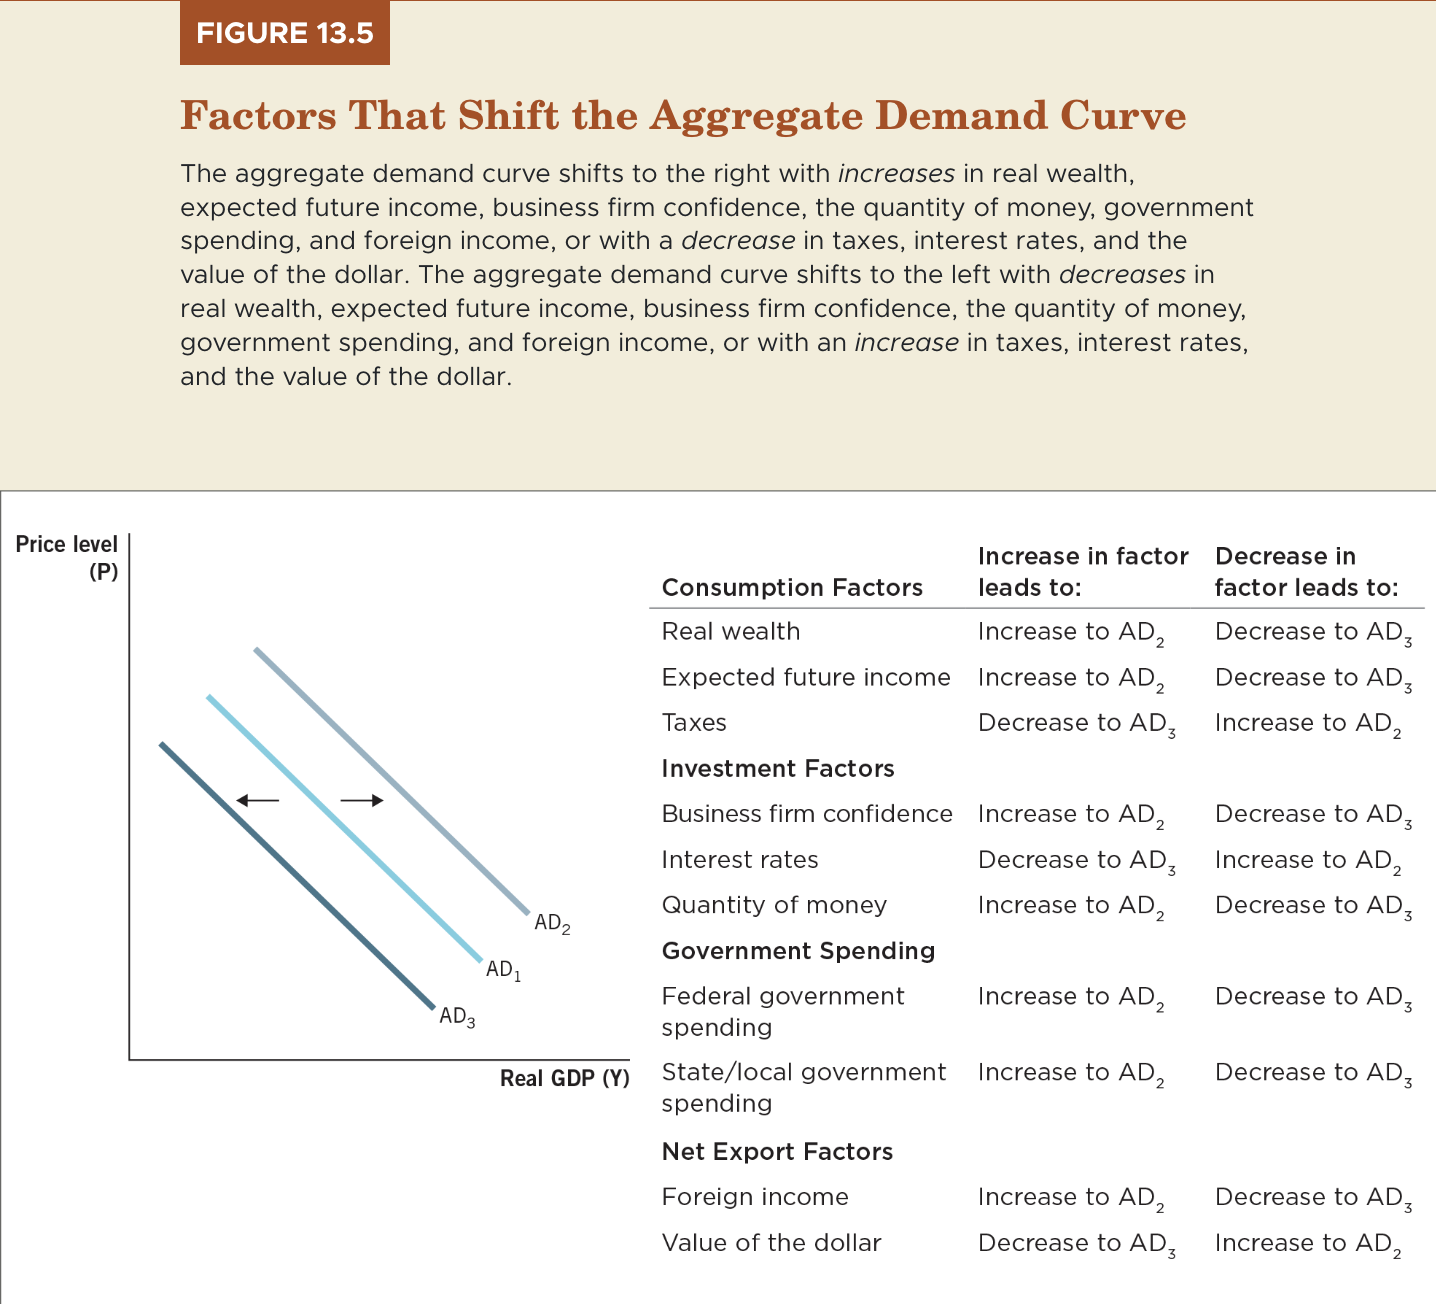
\includegraphics[scale=0.33]{images/Figure 13.5.png} 
\end{center}

Figure 13.5 summarizes the effects on the four categories of factors that shift aggregate demand; on the graph, initial aggregate demand is shown as \(\text{AD}_1\). Aggregate demand shifts to the right (to \(\text{AD}_2\)) with \textit{increases} in consumption, investment, government spending, or next reports. In contrast, aggregate demand shifts to the left (to \(\text{AD}_3\)) with \textit{decreases} in consumption, investment, government spending, or net exports.

\section*{\textbf{What is aggregate supply?}}
We have seen that aggregate demand embodies the spending desires of an economy. It tells us how many goods and services people want to buy at different price levels, but peoples' wants and desires alone do not determine GDP. We must also consider the supply side of the economy, which tell us about the willingness and ability of producers to supply GDP.

\begin{center}
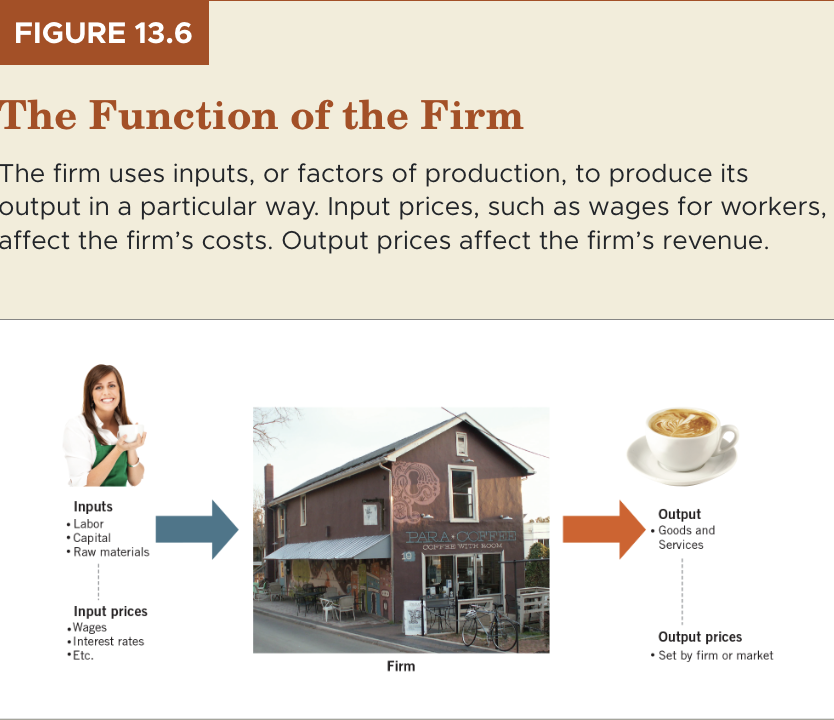
\includegraphics[scale=0.5]{images/Figure 13.6.png} 
\end{center}

Most of us relate easily to the demand side because we buy things all the time. To understand the supply side, we need to consider the perspective of those who produce and sell goods and services.

\textbf{\textit{Figure 13.6 presents an overview of the basic function of the firm.}}

To understand aggregate supply, we need to consider how changes in the overall price level (P) affect the supply decisions of the firm; but the influence of the price level on aggregate supply depends on the time frame. The \textbf{long run} in macroeconomics is a period of time sufficient for all prices to adjust. The long run doesn't arrive after a set period of time; it arrives when all prices have adjusted. In the \textbf{short run}, some prices change but others take more time; in macroeconomics, the short run is the period of time in which some prices have not yet adjusted.

\subsection*{Long-run aggregate supply (LRAS)}
As we've discussed several times in this text, the long-run output of an economy depends on resources, technology, and institutions. The short run may bring fluctuations in real GDP, but in the long run the economy moves toward full-employment output (\(Y\)*). The price level does not affect long-run aggregate supply; think of it this way: in the long run, the number of paper dollars we exchange for our goods and services does not affect our ability to produce.

Figure 13.7 plots the economy's long-run aggregate supply curve (LRAS). Notice that since we plot LRAS with the economy's price level (P) on the vertical axis and real GDP (Y) on the horizontal axis, the long-run aggregate supply is a vertical line at \(Y\)*, which is full-employment output. In Chapter 7, we defined full-employment output as the output produced in the economy when unemployment (u) is at the natural rate (\(u\)*). This is the output level sustainable for the long run in the economy; because prices don't affect full-employment output, the LRAS curve is a vertical line at (\(Y\)*). If the price level is 100, the quantity of aggregate supply is equal to \(Y\)*; if the price level rises to 110 or falls to 90, output in the long run is still \(Y\)*.

\subsubsection*{Shifts in the long-run aggregate supply}
The long-run aggregate supply curve shifts when there is a long-run change in a nation's ability to produce output, or a change in \(Y\)*. The factors that shift long-run aggregate supply are the same factors that determine economic growth: resources, technology, and institutions.
\begin{center}
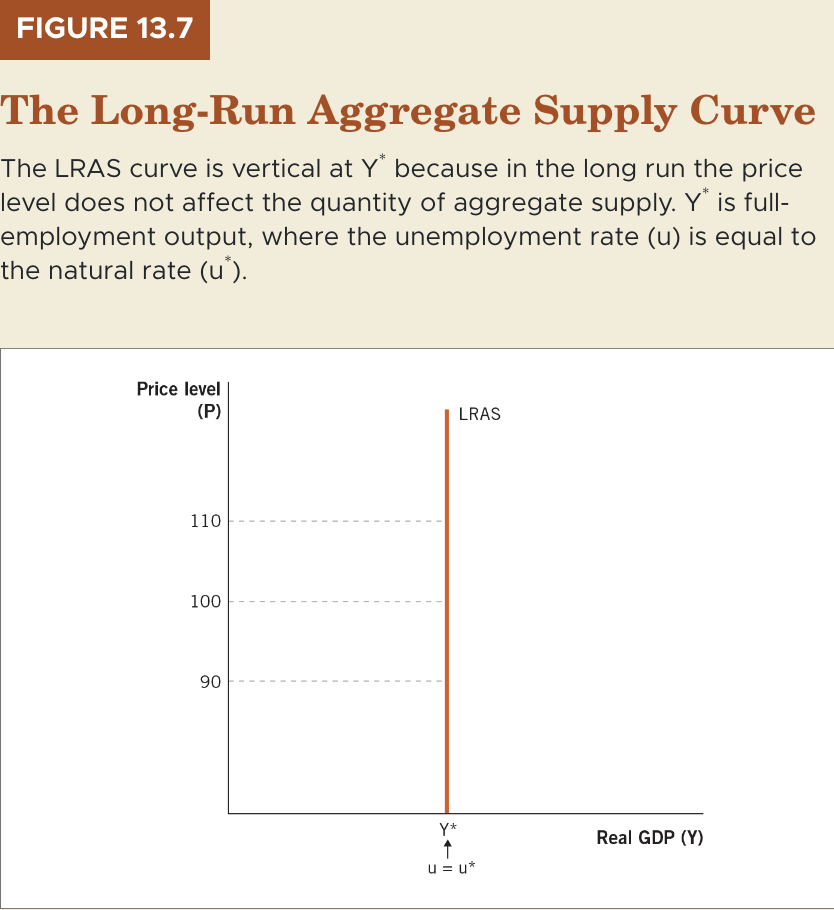
\includegraphics[scale=0.52]{images/Figure 13.7.png} 
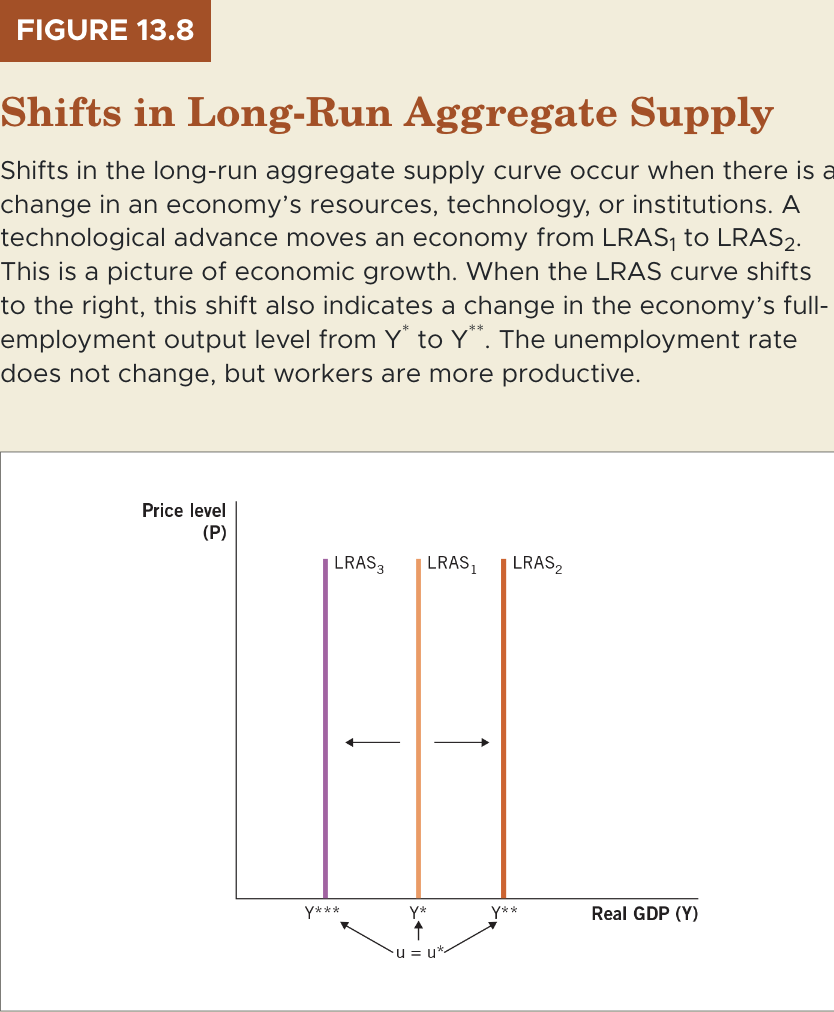
\includegraphics[scale=0.5]{images/Figure 13.8.png}
\end{center}

Figure 13.8 illustrates a shift in long-run aggregate supply; initially, the LRAS curve is vertical at \(Y\)*, which depends on resources, technology, and institutions. After the new driverless technology is introduced, \(\text{LRAS}_1\) shifts to the right (to \(\text{LRAS}_2\)) because now the full-employment output in the economy is greater than before. Notice that both before and after the shift, the unemployment rate is at the natural rate (\(u\)*). The new technology does not reduce the unemployment rate, but workers in the economy are more productive; the new output rate, (\(Y\)**), is designated with two asterisks because it represents a new full-employment output rate.

In previous chapters, we have used other models to illustrate economic growth by shifting out the economy's production possibilities frontier (PPF) or shifting up the aggregate production function. We illustrate economic growth in the AD-AS model using the long-run aggregate sup[ply curve. As the economy grows over time, full-employment output increases, shifting the LRAS curve to the right.

\subsection*{Short-run aggregate supply (SRAS)}
We just saw that the price level does not affect aggregate supply in the long run. However, in the short run there is a positive relationship between the price level and the quantity of aggregate supply. We consider three reasons for this relationship: inflexible input prices, menu costs, and money illusion.

First, consider input prices; one common input price is worker's wages, and these do not adjust quickly. For example, at your coffee shop, you pay a baristas a particular wage, and this wage is set for a period of time. In addition, interest rates for your business loans are normally fixed; economists say these inputs are \textit{sticky}, because they "stick" at a certain level and take time time to change. In contrast, output prices (like the price of the coffee beverages) are more flexible. Whereas input prices are often set by written contract, output prices generally easy to change; in a neighborhood coffee shop, prices are often written on a chalkboard, making them very easy to change from day to day.

The distinction between sticky input prices and flexible output prices is at the center of our discussion of aggregate supply; because it affects the way firms react when prices do move. Therefore, your costs remain the same; and here is the link to aggregate supply: because your costs don't rise but your revenues do, it makes sense for you to increase output. When you and other firms raise output, GDP rises.

The dynamic between sticky input prices and flexible output prices explains the positive slope of the short-run aggregate supply curve. Figure 13.9 shows the short-run aggregate supply curve, labeled as SRAS; when the price level rises from 100 to 110, firms produce more in the short run because input prices are sticky, and real GDP rises from \$20 trillion to \$21 trillion. When the price level falls to 90, firms produce less in the short run because flexible output prices fall but sticky input prices stay relatively high. The result is a decrease in real GDP to \$19 trillion.

\begin{center}
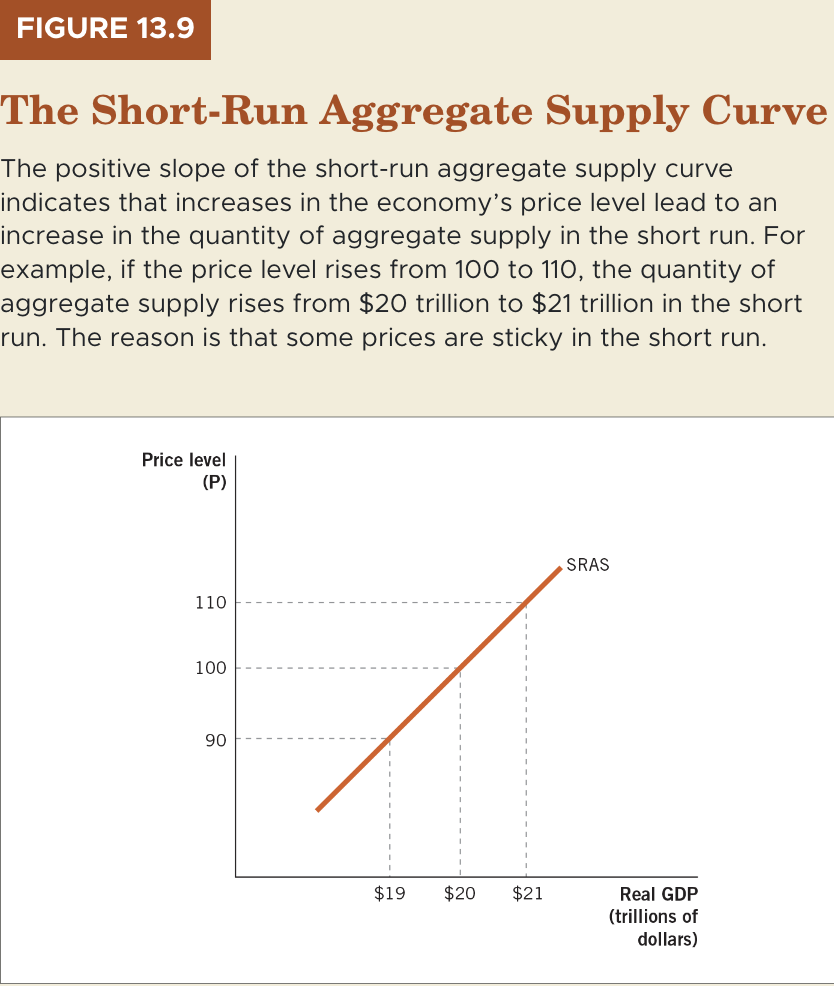
\includegraphics[scale=0.45]{images/Figure 13.9.png} 
\end{center}

There are other reasons why aggregate supply might be positively related to the price level in the short run. Menu costs, which we introduced in Chapter 8, are another factor that affects short-run aggregate supply; if the general price level is rising but a firm decides not to adjust its prices because of menu costs, customers will want more of its output. If firms decide to increase output rather than print new menus, the quantity of aggregate supply increases, so again, output is positively related to the price level in the short run.

We also talked about the problem of money illusion in Chapter 8. Recall that \textit{money illusion} occurs when people interpret nominal values as real values; in terms of aggregate supply, if output prices are falling but workers are reluctant to accept nominal pay decreases, they reinforce the stickiness of input prices. If input prices don't fall with output prices, firms reduce output in response to general price-level changes.

Any type of price stickiness leads to a positively sloped aggregate supply curve in the short run, but keep in mind that since all prices can change in the long run, the long-run aggregate supply curve is vertical at the full-employment output level.

\subsubsection*{Shifts in short-run aggregate supply}
When the long-run aggregate supply curve shifts, it signals a change that affects the economy in both the long run and the short run. Therefore, all long-run aggregate supply curve shifts (caused by changes in resources, technology, and institutions) also cause the short-run aggregate supply curve to shift; but, in addition, the short-run aggregate supply curve sometimes shifts on its own. Typically, these shifts are due to changes that directly affect firms' costs of production and form their incentives for supply.

The primary cause of shifts in short-run aggregate supply in changes in input or resource prices. Aggregate supply is the total quantity of GDP supplied by firms in the economy, as it relates to the overall price level. When input costs fall, production costs fall, and then firms produce more output at any given price level; this means short-run aggregate supply increases, or shifts to the right. The short-run aggregate supply curve exists because input prices and other prices are sticky and do not always adjust immediately when aggregate demand shifts; so when these prices do change, the short-run aggregate supply curve shifts. When input prices rise, short-run aggregate supply declines (the curve shifts to the left).

Although input price can change for many reasons, we will cover just two main ones. The first is a change in workers' wages; where workers are unionized, the unions engage in collective bargaining that leads to wage agreements between the workers as a group and their employers. If workers underestimated inflation in the past, this will inform their negotiations for higher wages in the future.

Along these same lines, if you are going to sign a long-term wage contract by yourself, you'll probably also form some expectation about future prices. After all, the real value of your future income depends on prices in the future; all else equal, when workers and firms expect higher prices in the future, they negotiate higher wages. The result is higher labor costs, which reduce firms' profitability and make them less willing to produce at any price level; therefore, higher expected future prices lead to a lower aggregate supply. The process works in reverse if workers and firms expect a lower price level; subsequent negotiation produce a labor agreement with lower wages, which reduces labor costs. When labor costs fall, additional production is more profitable at any price level, and the short-run aggregate supply curve shifts to the right.

A second cause of short-run aggregate supply shifts is \textit{supply shocks}. Sometimes, exogenous surprise events occur that change firms' production costs and shift aggregate supply; \textbf{supply shocks} are surprise events that change firms' production costs.

When supply shocks are temporary, they shift only the short-run aggregate supply curve; supply shocks can be negative or positive; (think about all the businesses reopening after worst of the pandemic was over.) Negative supply shocks lead to higher input prices and higher productions costs, shifting the short-run aggregate supply curve to the left. Positive supply shocks reduce input prices and production costs, shifting the short-run aggregate supply curve to the right.

\textbf{\textit{A price change in an important factor of production is another supply shock.}}

Figure 13.11 shows how changes in input prices shift the short-run aggregate supply curve; short-run aggregate supply increases (the curve shifts to the right to \(\text{SRAS}_2\)) when resource prices fall. This could occur when negotiation leads to lower worker wages or when there is a positive supply shock; short-run aggregate supply decreases (the curve shifts to the left to \(\text{SRAS}_3\)) when resource prices rise. This happens when workers negotiate higher wages or when negative supply shocks increases resource prices.

\begin{center}
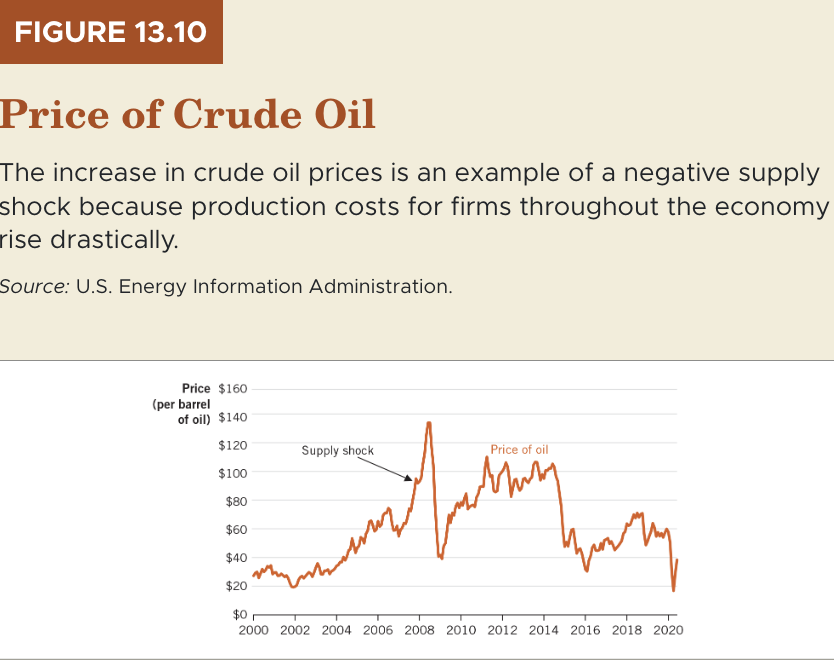
\includegraphics[scale=0.5]{images/Figure 13.10.png}
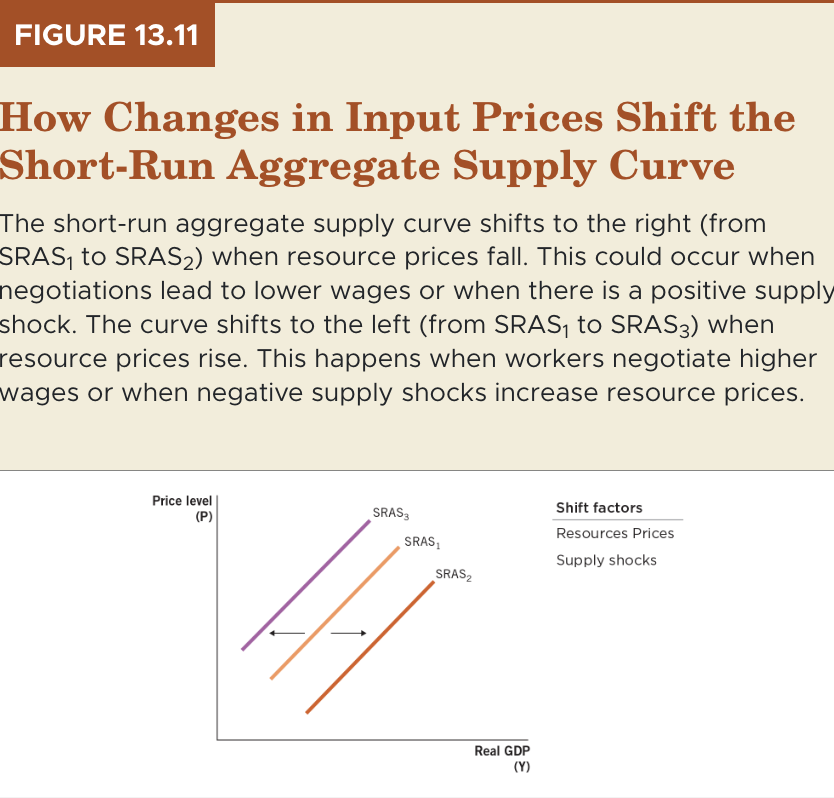
\includegraphics[scale=0.5]{images/Figure 13.11.png} 
\end{center}

\section*{\textbf{How does the Aggregate Demand-Aggregate Supply Model help us understand the economy?}}
In a market economy, output determined by exchanges between buyers and sellers, which are represented in our model by aggregated demand and aggregate supply. In this section, we bring aggregate demand and aggregate supply together and also consider how changes in the economy affect real GDP, unemployment, and the price level. As we are about to see, the economy tends to move to the point at which aggregate demand and aggregate supply are equal.

\subsection*{Equilibrium in the aggregate demand-aggregate supply model}
Figure 13.12 plots aggregate demand and aggregate supply curves on the same axes. The point where they intersect, A, is the equilibrium point where the opposing forces of supply and demand are balanced. At point A, the price level is \(P\)* and the output level is \(Y\)*; prices naturally adjust to move the economy toward the equilibrium point.

To understand why the economy tends toward equilibrium at price level \(P\)*, consider other possible price levels. For example, at price level \(P_H\), which is higher than \(P\)*, aggregate supply is greater than aggregate demand; here firms produce more than consumers desire at current prices. Therefore, prices naturally begin to fall to eliminate a potential surplus of goods and services; as prices fall, the quantity of aggregate demand increases and the economy moves towards a new equilibrium at \(P\)*.

In contrast, if the price level is \(P_L\) which is lower than \(P\)*, aggregate demand exceeds aggregate supply. At \(P_L\), buyers desire more than producers willing to supply; because aggregate demand exceeds aggregate supply, prices rise and the price level moves toward \(P\)*. The only price level where the plans of suppliers and demanders match is \(P\)*. Market forces automatically push the economy to the price level where aggregate demand equals aggregate supply.

\begin{center}
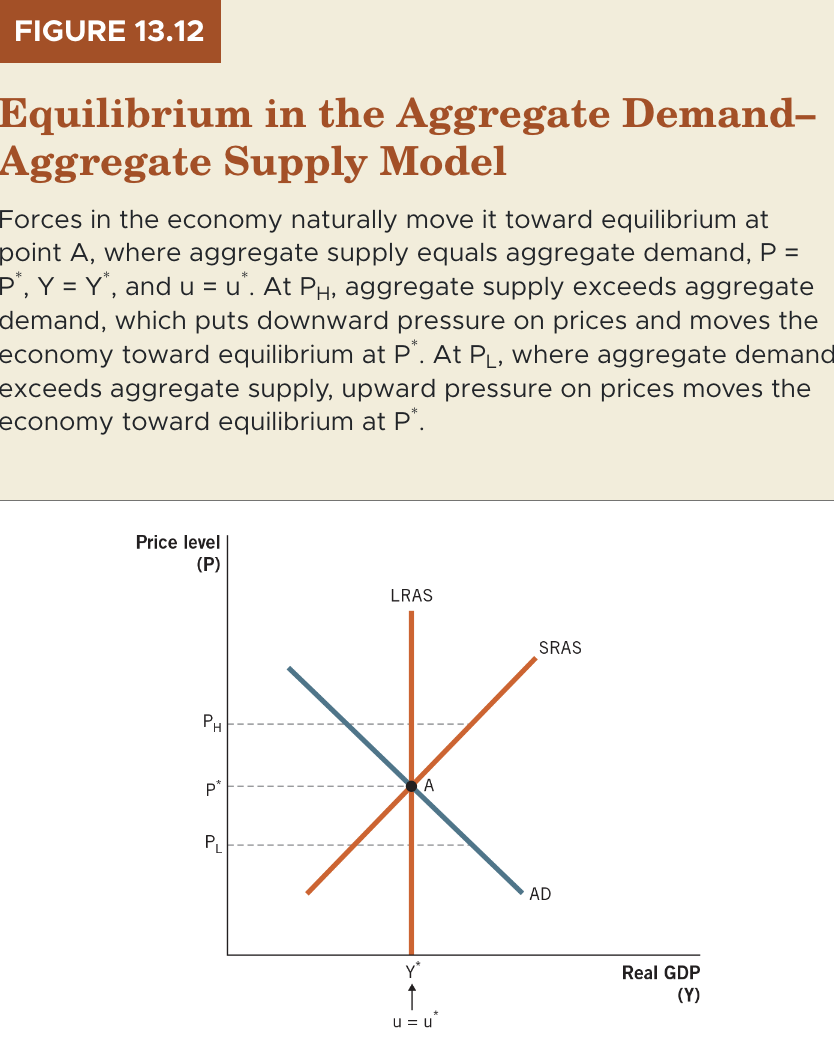
\includegraphics[scale=0.35]{images/Figure 13.12.png} 
\end{center}

We can also describe this equilibrium in equation form; in equilibrium, both long-run and short-run aggregate supply are equal to aggregate demand:
\begin{equation}
\text{LRAS}=\text{SRAS}=\text{AD}
\end{equation}
Aggregate supply is the real GDP produced, which we indicate as Y. Aggregate demand derives from four components: C, I, G, and NX; therefore, we can rewrite equations 13.2 as:
\begin{equation}
Y=C+I+G+\text{NX}
\end{equation}
Now we know what equilibrium looks like in our model; the second equation is our reference point for thinking about the economy at a particular point in time.

But the real world begins constant change: everything from technology to weather to wealth and expectations can change. Now that we've built our model of the macroeconomy, we can examine how real-world changes affect the economy.

In what follows, both in this chapter and for the remainder of the book, we consider many real-world factors that lead to changes in the macroeconomy. When we consider a change, we follow a particular sequence of steps to the new equilibrium. Once we determine the new equilibrium, we can assess the effects of the changes on real GDP, unemployment, and the price level. The five steps are as follows:
\begin{enumerate}
\item Begin with the model in long-run equilibrium.
\item Determine which curve(s) are affected by the change(s), and identify the direction(s) of the changes(s).
\item Shift the curve(s) in the appropriate direction(s).
\item Determine the new short-run and/or long-run equilibrium points.
\item Compare the new equilibrium point(s) with the starting point.
\end{enumerate}
Next we consider shifts in all three curves: long-run aggregate supply, short-run aggregate supply, and aggregate demand.

\subsection*{Adjustment to shifts in long-run aggregate supply}
Let's begin with shifts in the long-run aggregate supply curve. We have seen that technological advances increases full-employment output and shift the long-run aggregate supply curve to the right. For example, the Internet is a relatively new and important technology, made available to the general public in the 1990s. The Internet makes millions of workers more productive; the effect on overall economy is illustrated in Figure 13.13

\begin{center}
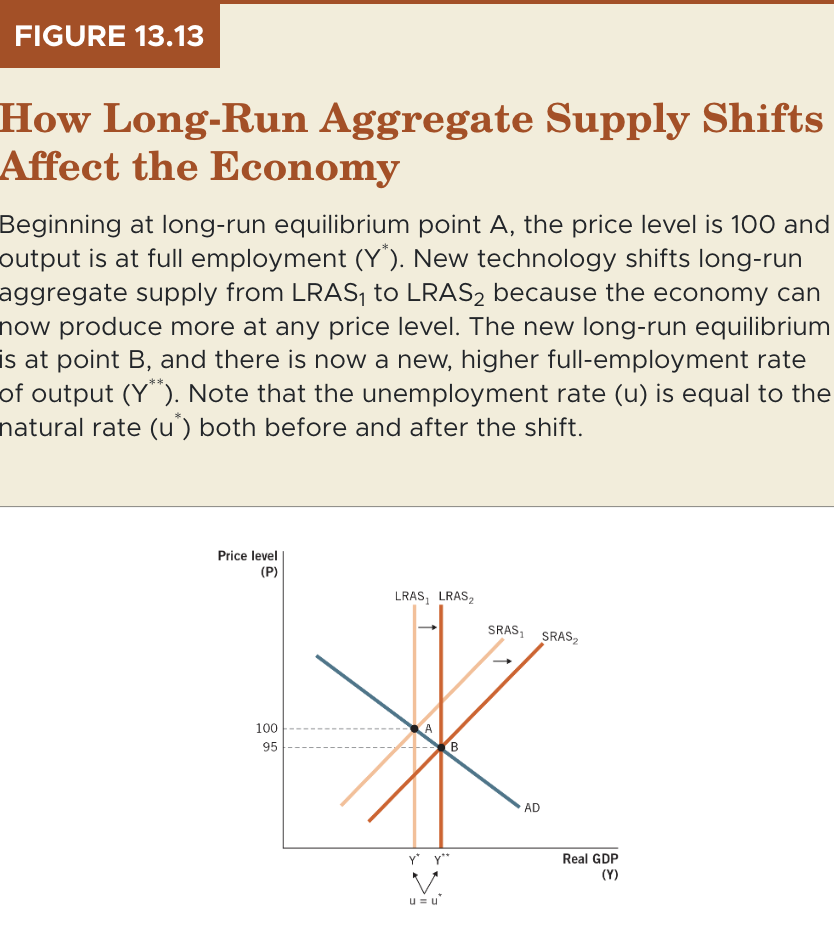
\includegraphics[scale=0.5]{images/Figure 13.13.png}
\end{center}

All else equal, technological progress leads to more output and a lower price level, which drops from 100 to 95. Before the Internet, the unemployment rate was at the natural rate (\(u\)*); after the new technology becomes available, employment remains at \(u\)*; but better tools mean workers can produce more output (\(Y\)** vs. \(Y\)*). This also applies to other factors that shift long-run aggregate supply to the right, such as the discovery of new resources or the introduction of new institutions favorable to growth.

\subsection*{Adjustments to shifts in short-run aggregate supply}
Now let's consider a change in short-run aggregate supply; one possibility is a short-run supply disruption caused by an oil pipeline break, a negative supply shock. Because oil is a widely used input, the disruption temporarily raises production costs. We show this supply shock in Figure 13.14 by shifting short-run aggregate supply to the left, from \(\text{SRAS}_1\) to \(\text{SRAS}_2\); this new equilibrium is at point b, with a higher price level (105) and lower level of output (\(Y_1\)). Because this is a short-run equilibrium, we use the lowercase b; the lower output means increased unemployment in the short run (\(u > u\)*). Notice that nothing happens to long-run aggregate supply - in the long run, the pipeline is fixed and oil is produced at full-employment output level \(Y\)* again.

\begin{center}
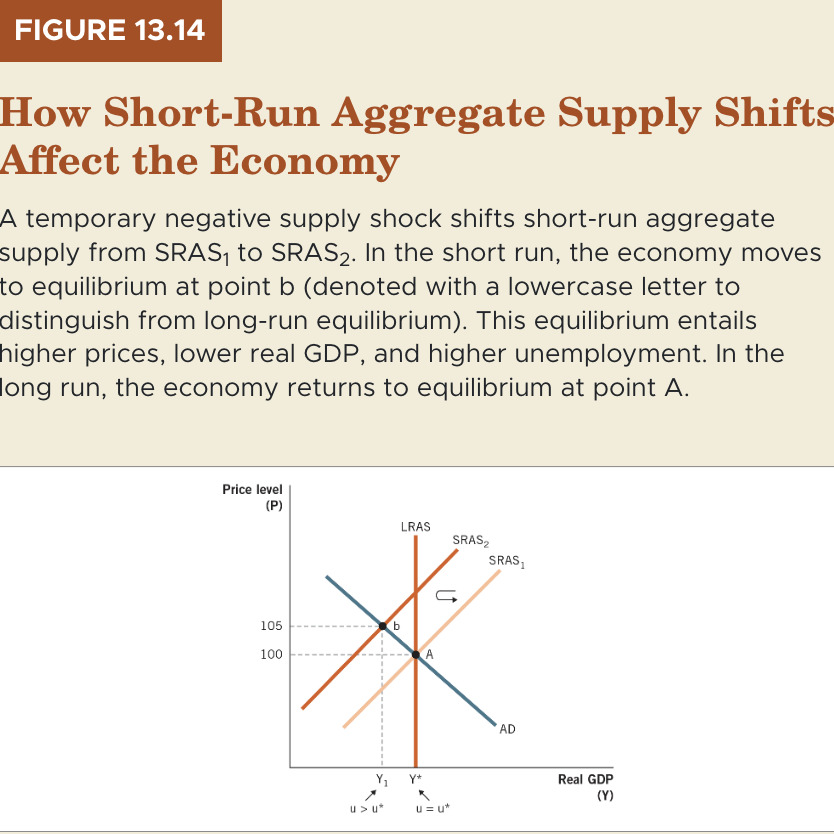
\includegraphics[scale=0.5]{images/Figure 13.14.png} 
\end{center}

Because the disruption is temporary, eventually the short-run aggregate supply curve shifts back to the right until it reaches \(\text{SRAS}_1\) again. Short-run disruptions in aggregate supply do not alter long-run equilibrium in the economy; eventually, the price level, output, and unemployment rate return to their long-run equilibrium levels at point A. But in the short run, the negative shift brings higher unemployment and lower real GDP.

\subsection*{Adjustments to shifts in aggregate demand}
Aggregate demand shifts for many reasons; shifts might even occur from changes in expectations of market participants rather than from real factors in the economy, and yet even these subjective factors affect the macroeconomy. For example, consider an unexpected change in consumer confidence: consumers wake up one morning with expectations of higher future income. This then increases aggregated demand as consumers spend more; can this kind of change have real effects on the economy? That is, will a change in consumer confidence affect unemployment and real GDP? Let's look at the model.

\begin{center}
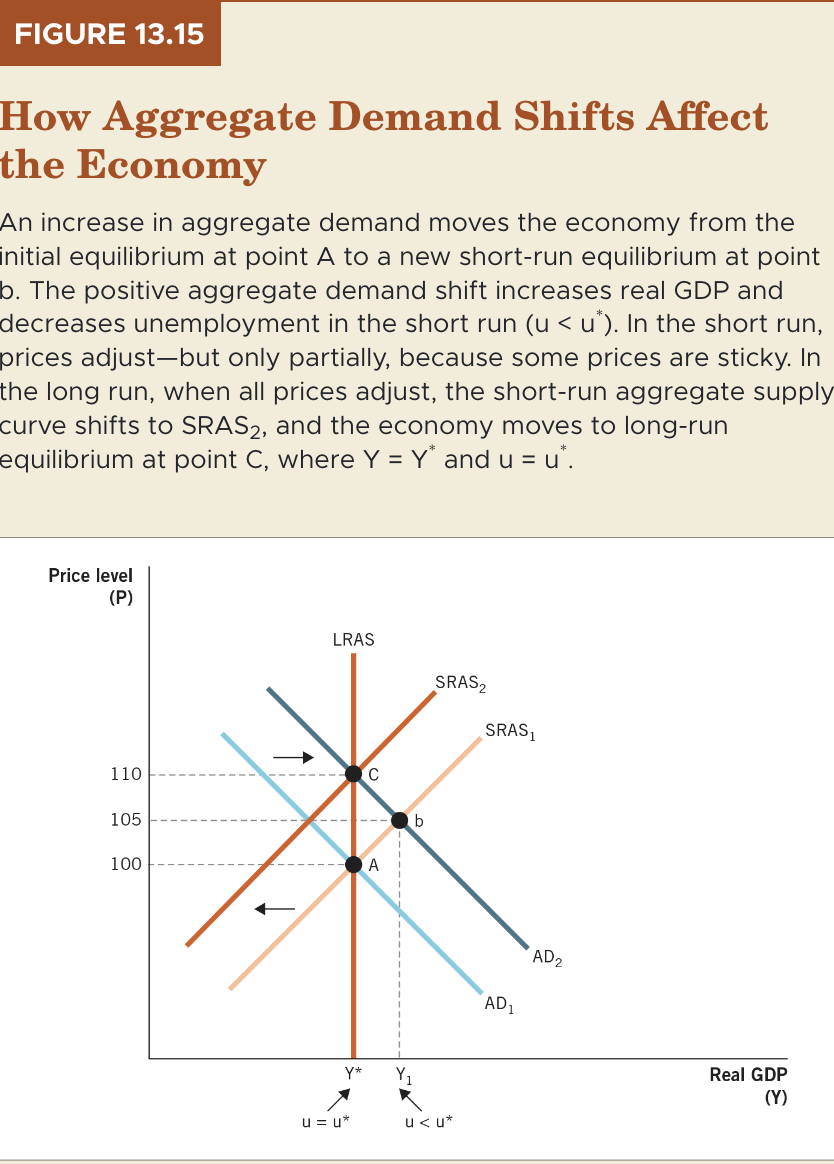
\includegraphics[scale=0.45]{images/Figure 13.15.png}
\end{center}

Figure 13.15 illustrates changes in the economy from an uptick in consumer confidence. We start in long-run equilibrium at point A, where the price level of 100, real GDP is at full-employment output \(Y\)*, and unemployment is equal to the natural rate (\(u = u\)*). More spending means aggregate demand shifts from \(\text{AD}_1\) to \(\text{AD}_2\), and the economy moves to short-run equilibrium at point b. The short-run equilibrium is relevant here, because in the short run some prices are sticky, so that even though there is upward pressure on prices, only some prices adjust and the price level rises to 105. But this short-run equilibrium is also associated with higher real GDP (\(Y_1\)) and an unemployment rate of \(u_1\), which is less than the natural rate, \(u\)*. Thus, changes in aggregate demand do affect the real economy (Y and u), at least in the short run.

Our initial results seem very positive - after all, unemployment falls and real GDP rises in the short run; but we need to complete the story by following through to long-run equilibrium. Recall the difference between long run and the short run: in the long run, all price adjust; as all prices adjust, short-run aggregate supply shifts back from \(\text{SRAS}_1\) to \(\text{SRAS}_2\). The economy then moves to long-run equilibrium at point C; notice that at C we are back to the original output level (\(Y\)*) and unemployment level (\(u\)*), but prices are higher (\(P = 100\)). The model is telling us that demand changes have no real effects (on Y and u) in the long run as only the price level (a nominal variable) is affected.

\begin{center}
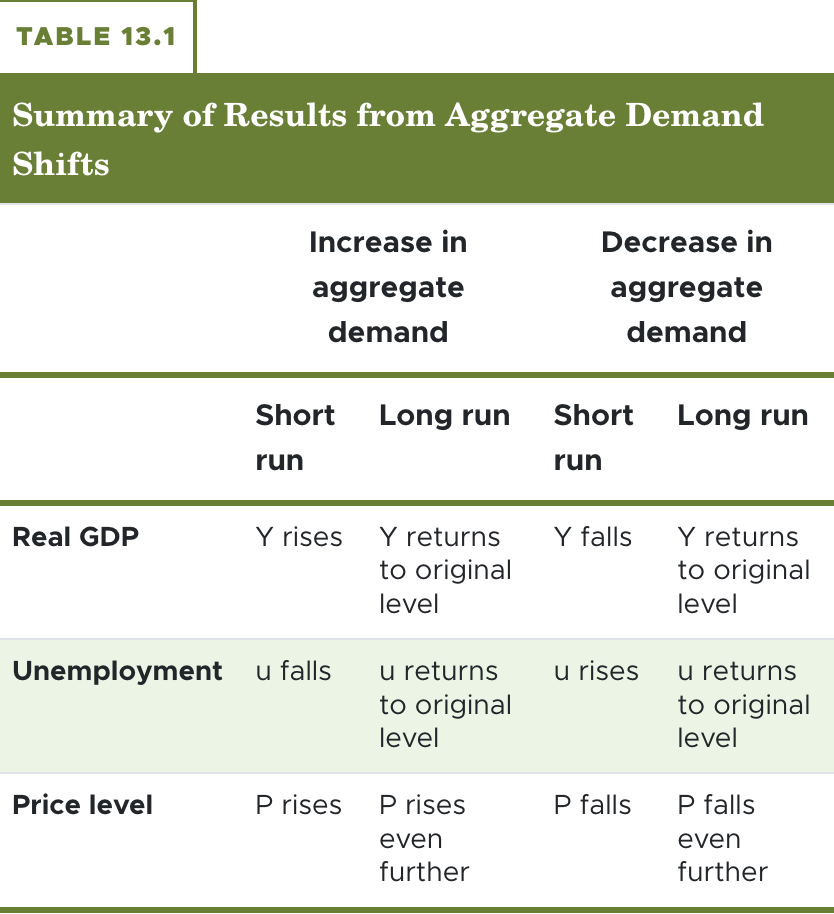
\includegraphics[scale=0.5]{images/Table 13.1.png} 
\end{center}

What are the consequence of this move to long-run equilibrium, and how does it compare with the short-run equilibrium? At point b, real GDP is up and unemployment is down; but not everyone is happy.

But since all prices can adjust eventually, the economy moves to point C in the long run. When input prices rise to match output price changes, the short-run aggregate supply curve shifts to \(\text{SRAS}_2\). In the long run, after all prices have adjusted, the price level does not affect the quantity of output supplied; this is why output returns to \(Y\)*, the full-employment level.

Table 13.1 summarizes the economic effects of aggregate demand changes in both the short run and the long run. The last two columns summarize the effects of decreases in aggregate demand; these decreases in aggregate demand are a particular source of debate among macroeconomists. We'll examine the historical effects of changes in aggregate demand in Chapter 14.

\section*{\textbf{Conclusion}}
We began this chapter with the misconception that recessions are regular occurrences that happen every few years. In fact, they are anything but certain or predictable; they occur with unpredictable frequency and are caused by many different factors. Recessions in business cycles are often caused by changes in aggregate demand, but the same symptoms can also reflect short-run aggregate supply shifts.

This chapter introduced the aggregate demand-aggregate supply model of the economy, which helps us understand how changes in the real world affect the macroeconomy. In the next chapter, we use the model to evaluate three biggest macroeconomic disturbances of the past century: the Great Depression of the 1930s; the Great Recession of 2007-2009; and the most recent recession, caused by COVID-19.
\end{document}